We now show an approximation-preserving reduction from \ProbGroup{} to
\Prob{}.
Given an instance of \ProbGroup{}, $(G, w, S, \mathcal{G})$, where $G = (V, E)$, 
we define an instance of \Prob{},
$(G', w')$ where $G' = (V', E')$, and:
\begin{description}
\item[V'] - $V \cup \mathcal{G}$
\item[E'] - $E \cup \{vg_i : v \in g_i\} \cup (V \times V) \setminus E$
\item[w'] - $
w'(e) = 
\begin{cases}
w(e) 	& e \in E
\\
\infty & \text{otherwise}
\end{cases}
$
\end{description}


\begin{figure}
\begin{center}
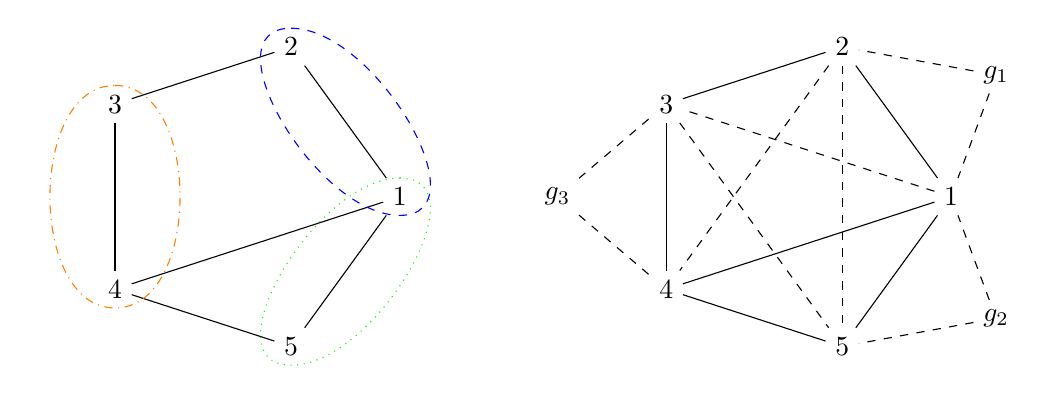
\begin{tikzpicture}[]
\foreach[count=\i] \a in {0,72,...,288}{
	\node(\i) at(\a:2) {\i};
}

\foreach \u \v in {
	1/2,2/3,3/4,4/1,4/5,5/1%
}{
	\draw (\u) -- (\v);
}

\draw[dashed, blue]
(2.north) to[out=0,in=0]
(1.south) to[out=180,in=180]
(2.north)
;

\draw[dotted, green]
(1.north) to[out=0,in=0]
(5.south) to[out=180,in=180]
(1.north)
;

\draw[dash dot, orange]
(3.north) to[out=0,in=0]
(4.south) to[out=180,in=180]
(3.north)
;

\begin{scope}[xshift=7cm]
\foreach[count=\i] \a in {0,72,...,288}{
	\node(\i) at(\a:2) {\i};
}

\foreach \u \v in {
	1/2,2/3,3/4,4/1,4/5,5/1%
}{
	\draw (\u) -- (\v);
}

\node(g1) at(31:3){$g_1$};
\node(g2) at(-31:3){$g_2$};
\node(g3) at(180:3){$g_3$};

\foreach \u \v in {
	1/3%
	,2/4,2/5%
	,3/5%
	%
	,g1/1,g1/2%
	,g2/1,g2/5%
	,g3/3,g3/4%
}{
	\draw[dashed] (\u) -- (\v);
}
\end{scope}

\end{tikzpicture}
\end{center}
\caption{\label{fig:prob-geq-group}
From left to right:
a) An instance of \ProbGroup{} (weights are omitted), 
groups are marked by a dashed blue, dotted green, and dashed-dotted lines respectively.  
b) A corresponding \Prob{} instance: we add a vertex for each group and connect it 
to all terminals in the group.
Weights for the original edges remain intact, dashed edges have infinity weight.   
}
\end{figure}

\begin{claim}
Any dominating tree with finite weight, $T$, in $(G', w')$ is a feasible group Steiner tree in 
$(G, w, S, \mathcal{G})$.
\end{claim}

\begin{proof}
Observe first that $T$ contains only original edges or otherwise its weight is infinite.  
Assume for contradiction that $T$ is not feasible group Steiner tree, that is, there is 
a group $g_i$ such that none of the vertices in $g_i$ is spanned by $T$, that is $g_i$
is not in dominated by any vertex in $T$ - contradiction. 
\end{proof}
 
\begin{claim}
Any feasible group Steiner tree in $(G, w, V, \mathcal{G})$, $T$, is a dominating tree
in $(G', w')$.
\end{claim}

\begin{proof}
First, observe that any original vertex dominate all other original vertices.
Assume for contradiction that $T$ is not a dominating tree, that is, there is 
a new vertex $g_i$ that is not dominated by $T$ which implies that 
$T$ does not cover $g_i$ - contradiction. 
\end{proof}